Das Architekturdiagramm zeigt eine klassische Client-Server-Architektur, die in zwei Hauptbereiche unterteilt ist: Frontend und Backend. 
Im Frontend-Bereich befinden sich mehrere Komponenten: die Hauptwebsite "rf-innotrade.de" sowie beliebig viele Unterwebseiten (hier: Subbrands). Jede dieser Frontend-Komponenten kommuniziert mit dem Backend über HTTP-Requests und erhält entsprechende HTTP-Responses zurück. 
Das Backend, besteht aus einer Strapi-Anwendung als zentraler Komponente. Diese ist mit einer SQLite-Datenbank verbunden, die für die Datenspeicherung zuständig ist. Zusätzlich ist eine Shopify-Instanz eingebunden. Diese einbindung erfolgt über einen sogenannten Buy Button, welcher durch ein von Shopify selbst erzugtes Skript auf die Unterwebseiten eingebettet wird. Dieses Skript kommuniziert mit Shopify und bildet darüber diverse Shopfunktiuonen ab.
Die gesamte Architektur folgt einem einheitlichen Kommunikationsmuster, bei dem alle Frontend-Komponenten über standardisierte HTTP-Verbindungen mit dem Strapi-Backend interagieren. Diese klare Trennung zwischen Frontend und Backend ermöglicht eine skalierbare und leicht zu wartende Systemarchitektur\vglfootcite{rajabov_role_2023}.

\begin{figure}[H]
    \centering
    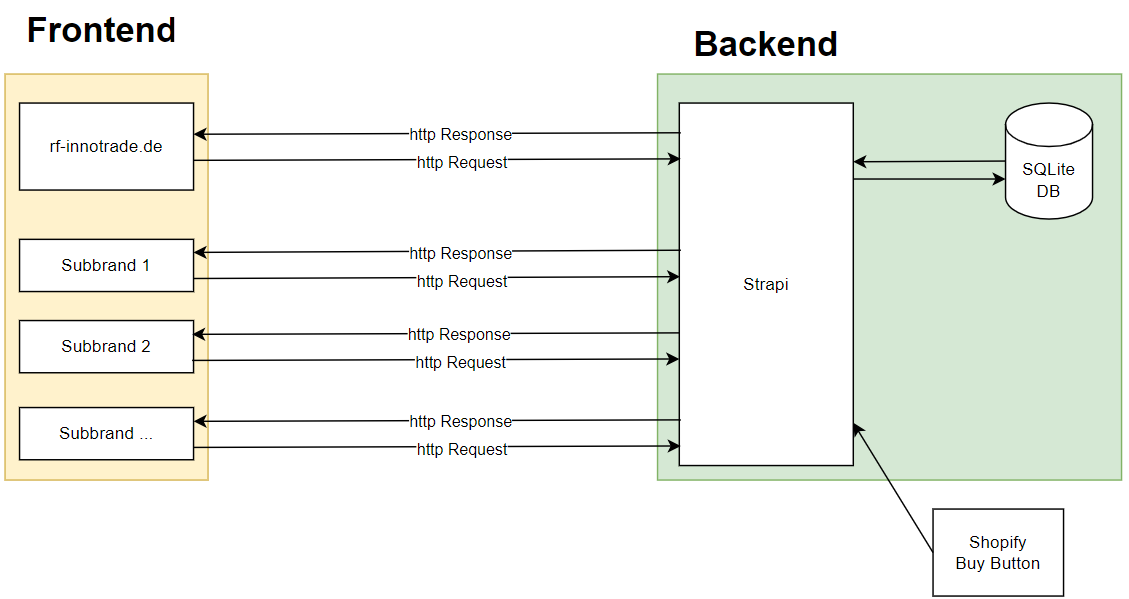
\includegraphics[width=1\textwidth]{figures/architektur.png}
    \caption{Architektur Schaubild, Quelle: Eigene Darstellung}
	\label{fig:architekturSchaubild}
\end{figure}